\documentclass{article}

%% Denote paragraphs with vertical space rather than indenting (not critical)
\usepackage{parskip}

%% Support for URL in introductory text (not needed for main example)
\usepackage{url}

%% *** Enable TikZ ***
\usepackage{tikz}


\begin{document}

%% Introductory Text
Example 3.10 from the book\\
\emph{Unlocking LaTeX Graphics: A Concise Guide to Ti$k$Z/PGF and PGFPLOTS}.\\
For more information, visit \url{https://latex-graphics.com}.
\par\bigskip

%% *** START OF EXAMPLE CODE ***
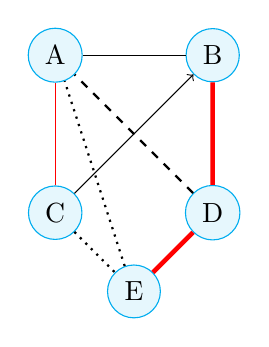
\begin{tikzpicture}[every node/.style={circle, draw=cyan, fill=cyan!10}]
  \path (0,3) node (A){A} (2,3) node (B){B} (0,1) node (C){C} (2,1) node (D){D} (1,0) node (E){E};
  \draw (A.east) -- (B.west);
  \draw[->] (C.45) -- (B.225);
  \draw[red] (C.north) -- (A.south);
  \draw[thick,dotted] (C.315) -- (E.135)
    (E.110) -- (A.290);
  \draw[ultra thick,red] (D.north) -- (B.south) (E.north east) -- (D.south west);
  \draw[thick,dashed] (D.135) -- (A.south east);
\end{tikzpicture}
%% *** END OF EXAMPLE CODE ***

\end{document}
